\chapter{Háttérismeretek}\label{chap:hatter}

\section{Kapcsolódó munkák}
\label{sec:related-work}
\subsection{Gamma Statechart Composition Framework}
A Gamma Statechart Composition Framework\cite{gammaf} egy tanszéken fejlesztett eszköz, ami komponenst alapú viselkedés modellezést tesz lehetővé. Az eszköz képes kódot generálni és a formális verifikáció végrehajtani, továbbá képes Yakindu modelleket áttranszformálni Gamma modellekké. A Yakindu-Gamma transzformáció megvalósítása hasonló mint az általam implementált MagicDraw-gamma transzformáció. A Gamma keretrendszerrel \aref{sec:gamma-framework} szakasz foglalkozik részletesebben. 

\subsection{TismTool}

TismTool\cite{veugen2012framework} egy többszálú, komponens alapú rendszerek fejlesztését támogató eszköz, ami képes UML modellekből kódot generálni különböző nyelveken (C\#, Java, C++ vagy C) és ezeket verifikálni. Az eszköz képes különböző UML modellező eszközök modelljeit feldolgozni, az egyetlen megkötés, hogy ezek képesek legyenek az UML model XML Metadata Interchange (XMI) szabvány szerint modellt sorosítani: a MagicDrawra ez teljesül.

Az eszköz azáltal végzi el a verifikációt, hogy kódot generál az XMI fájlokból amit egy futtatókörnyezettel kell végrehajtatni továbbá nem formális alapokon hajtja végre a verifikációt, hanem ún. futás idejű verifikációt\footnote{http://www.tismtool.com/tooling.html} használ.
\section{Modellek}

Modelleket a tudomány számos területén alkalmazunk, ez lehetővé teszi az előtt vizsgálni a megvalósítandó rendszert, hogy azt ténylegesen létre kellene hozni. A vizsgálatoknak számos módja és célja lehet. A látványtervező bemutat egy látványtervet és a megfelelő \emph{stakeholderek} ezt értékelik, vagy egy rendszerről komplex matematikai módszerekkel kell eldönteni, hogy stabil-e. A modellek leírása sokféle módon történhet, de célszerű egy olyan standardizált jelölési rendszert alkalmazni, hogy a többi szakember is értelmezni, vizsgálni tudja a modellt.

A jelölési rendszer vagy modellezési formalizmus lehet egy szöveges leírás is, például egy programkód, de sokszor célszerű vizuális megoldást használni, szimbólumokat tartalmazó diagramokat alkalmazni. Ezek sok esetben kifejezőbbek, lényegre törőbbek, és elsősorban könnyebben értelmezhetőek mint a szöveges leírások.

\section{Állapot alapú modellezés}

Az állapottérkép egy diagram ami irányított gráfot tartalmaz, ahol a csomópontok állapotokat, az élek állapotátmeneteket definiálnak. Az így kapott gráfot állapotgépnek nevezzük. Az állapotátmenetek állapotok közötti lehetséges átjárásokat definiálnak és általában feltételhez kötöttek, ami jellemzően valamilyen esemény bekövetkezése vagy logikai feltétel teljesülése. A feltételek teljesülésekor az állapotváltás bekövetkezik, ezt szokás \emph{tüzelésnek} is hívni. Az állapotgép legfőbb jellemzője, hogy adott időpillanatban melyik állapotok aktívak. Állapotváltások aktív állapotból történnek, ilyenkor a kiindulási állapot inaktívvá válik a célállapot pedig aktívvá (a kiinduló és célállapot megegyezhet).

A működés kezdetekor az első aktív állapotot kezdő állapotnak hívják, ez egy különleges ún. pszeudoállapot, ami az állapotgép belépési pontja és általában azonnal átléptetésre kerül egy másik állapotba.

\subsection{Állapottérképek UML 2-ben}
Előzőekben az állapot alapú modellezés alapjai kerültek bemutatásra. A következőkben az állapottérképek egy konkrét specifikációja kerül bemutatásra az UML 2 szerint.

\begin{itemize}
	%--------------
	% Állapot
	%--------------
	\item \emph{Állapot (State)}: az állapottérképek csomópontjai, melyeket UML 2-ben is állapotoknak hívnak. Az állapotok rendelkeznek:
	\begin{itemize}
		\item név: az állapot neve
		\item be/kilépési akció: be és kilépés során végrehajtandó cselekvés.
	\end{itemize}
	
	%-----------------
	% Kezdő állapot
	%-----------------
	\item \emph{Kezdő állapot (Initial State)}: pszeudoállapot, régiónként egy szerepelhet belőle és a régió belépési pontjaként szolgál. Jelölése fekete színezett kör (\ref{fig:pseudo-and-final} ábra).
	%-----------------
	% Végső állapot
	%-----------------
	\item \emph{Végállapot (Final State)}\footnote{UML 2-ben a végső állapotot nem pszeudoállapotként hanem állapotként van definiálva https://www.omg.org/spec/UML/2.0} (final state): A végső állapot, a régió terminálasi pontja, ha egy állapotgép összes régiója egy végső állapotba ért akkor az állapotgép is terminál. Szimbóluma fehér körben egy kisebb színezett fekete kör (\ref{fig:pseudo-and-final} ábra).
	%----------------
	% Termináló állapot
	%----------------
	\item \emph{Termináló állapot (Terminal State)}: pszeudoállapot, ami az egész állapotgépet azonnal terminálja. Ezt hibák lekezelésére lehet például alkalmazni, jelölése kis kereszt (\ref{fig:pseudo-and-final} ábra).
	%--------------
	% Állapot átmenet
	%--------------
	\item \emph{Állapot átmenet (Transition)}: az állapottérképek élei, a lehetséges állapotváltozásokat definiálják. Az állapotátmenetek rendelkeznek:
		\begin{itemize}
			\item Triggerekkel
			\item Őrfeltételekkel
		\end{itemize}
	%---------------
	% Trigger
	%---------------
	\item \emph{Trigger}: Állapot váltást kiváltó esemény amely lehet:
	\begin{itemize}
		\item Változás esemény (Change Event): valamely változó értéknek a megváltozása.
		\item Üzenet esemény (Message Event): üzenet típusú objektumnak az érkezése, ami ebben a kontextusban kérésnek felel meg. Az ilyen típusú kommunikáció kétféle eseménytől függ, az üzenet elküldésétől és annak küldőjétől és az üzenet fogadásától és fogadójától. A kérés lehet egy metódus hívás vagy egy jel (\emph{Signal}) fogadása.
		\item Időzítés esemény (Time Event): idő változásához kötött esemény.
	\end{itemize}

\end{itemize}
Fontos megjegyezni, hogy a dolgozat nem tér ki részletesen az események kiváltásának kérdésére, valamint az események küldésénél és fogadásánál szerepet játszó portokra, és interfészekre, ezen elemek a dolgozat szempontjából irrelevánsnak tekinthetők.
\begin{itemize}
	%----------------
	% Guard
	%----------------
	\item\label{sec:guard} \emph{Őrfeltétel (Guard)}: tágabb értelemben egy logikai kifejezés, melynek teljesülnie kell, hogy az adott állapotátmenet bekövetkezhessen. UML-ben ezek megszoríráskén \emph{(Constraint)} vannak értelmezve, ebben az értelemben a megszorításnak való megfelelés az állapotváltás feltétele.
	%----------------
	%Action
	%----------------
	\item \emph{Akció}: Különböző események bekövetkezésekor, mint állapotváltások, belépés állapotokba, kilépés állapotokból, vagy maga az állapotban maradás, lehetőségünk van viselkedéseket végrehajtani. UML szerint ezek lehetnek: Activityk, Állapotgépek, Interakció\footnote{Interakció modell elemek között, leírásához a jellegétől függően többféle diagram használható(Szekvencia, Kommunikációs, Időzítés).} OpaqueBehavior\footnote{ szöveges, UML-től eltérő nyelvvel specifikált viselkedés.} Állapotváltáskor, állapotba való be-, kilépéskor a viselkedés végrehajtódik, míg állapotban maradáskor addig hajtódik végre, amíg az állapot aktív, egyébként megszakításra kerül.
	
	%-----------------
	% Ábra: állapot-atmenet-trigger-guard-action
	%----------------
	\begin{figure}[!ht]
		\centering
		
\includegraphics[keepaspectratio]{figures/statechart_elements/states.png}
		\caption{Állapotok és köztük definiált állapotátmenet, triggerrel, őrfeltétellel és actionnel}
	\end{figure}
	%----------------
	% Összetett állapot
	%----------------
\end{itemize}
Gyakran előfordul, hogy általánosabb állapotot célszerű felbontani részállapotokra. Az egyszerű állapottérképek elemeivel, ez a fajta hierarchikus viszony az állapotok között nehezen ábrázolható, ezért célszerű további elemek használata.
\begin{itemize}	
	%------------------
	% Régió
	%------------------
	\item \emph{Régió}: állapotokat tartalmazó egység, az állapottérkép mindig tartalmaz egy régiót amibe az állapotok definiálhatók. Régiók létezhetnek egymással párhuzamosan ilyenkor a végrehajtásuk párhuzamosan történik.
	%------------------
	% Öszetett állapot
	%-------------------
	\item \emph{Összetett állapot(Composite State)}: ha az állapotnak vannak további belső állapotai is, ha az állapot aktív akkor legalább egy belső is aktív, ha az állapotgép egy állapotváltás hatására kilép a kompozit állapotból akkor a belső állapotokból is kilép.
	%---------------
	% History state
	%--------------
	\item \emph{History State}: olyan pszeudo állapot, amely egy régióban megjegyzi az utolsó aktív állapotot kilépéskor. A régióba visszalépve a history state visszaállítja a megjegyzett állapotot. Amennyiben nincs előző állapot az ő belőle húzott állapotátmenet cél állapota lesz aktív. Kétféle History Statet különböztetünk meg Shallow és Deep Historyt. Előbbi csak adott régión belül jegyzi meg az állapotot míg utóbbi a tartalmazott régiók állapotait is megjegyzi és visszaállítja.
	
	A \emph{HistroyStatek} szintaktikája \aref{fig:pseudo-and-final} ábrán látható.
	
\end{itemize}

\begin{figure}[!ht]
	\centering
	
\includegraphics[keepaspectratio, width=80mm]{figures/pseudo-and-final.png}
	\caption{Kezdőállapot, DeepHistory, ShallowHistory, Termináló állapot és Végállapot}
	\label{fig:pseudo-and-final}
\end{figure}


Rendszerünket egy időpillanatban több egymástól független állapot is jellemezheti. Ezt a viselkedést párhozamos régiók alkalmazásával lehet leírni.
\begin{itemize}
	%------------------
	% Ortogonális állapot
	%------------------
	\item \emph{Ortogonális állapot (Orthogonal State)}: olyan összetett állapot ami két vagy több régiót tartalmaz.
	%---------
	% Fork
	%---------
	\item \emph{Fork}: pszeudoállapot, ami egy beérkező átmenetet szétbont több átmenetre, amiknek a cél állapotuk ortogonális régiókban találhatók. A kimenő átmeneteken nem lehet se trigger, sem pedig őrfeltétel.
	%---------
	% Join
	%---------
	\item \emph{Join}: pszeudoállapot, ami több beérkező átmenetet kapcsol össze eggyé. Az átmenetek ortogonális régiókból kell, hogy induljanak és nem lehet rajtuk trigger vagy őrfeltétel. A join szinkronizációs funkcionalitással bír: addig nem lehet tovább lépni belőle amíg minden beérkező átmenet végre nem hajtódott.
	
	\emph{Fork/Join} alkalmazásával ki tudjuk kényszeríteni, hogy részrendszereink elérjenek egy adott állapotot, mielőtt a végrehajtás folytatódhatna. Jelölésük \aref{fig:forkjoin} ábrán látható. 
	
	%------------
	% Ábra: fork - join
	%-----------
	\begin{figure}[!ht]
		\centering
		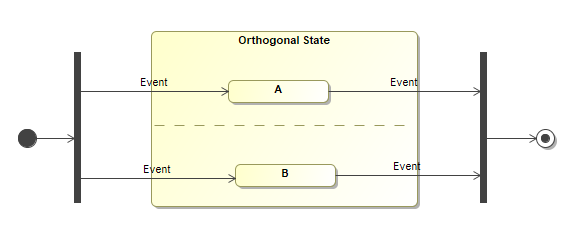
\includegraphics[keepaspectratio, width=100mm]{figures/statechart_elements/forkjoin.png}
		\caption{Példa: fork-join}
		\label{fig:forkjoin}
	\end{figure}
	
\end{itemize}
Rendszereink leírásakor előfordulhatnak ismétlődő részek, amiket célszerű egyszer leírni és újra felhasználni.
\begin{itemize}
	%-------------------
	% Submachine state
	%-----------------
	\item \emph{Submachine state}: Egy olyan állapot, ami egy állapottérképre hivatkozik, ez lehetővé teszi, hogy egy állapottérkép többszöri felhasználását, akár más-más kontextusban
	%---------------
	% Belépési pont
	%---------------
	\item \emph{Belépési pont(Entry Point)}: egy pszeudoállapot, ami egy állapotgép vagy egy kompozit állapot belépési pontját reprezentálja, célja egységbe zárni az állapotot vagy az állapotgépet. Továbbá léteznie kell egy állapotátmenetnek közte és egy az állapot vagy állapottérkép fő régiója között. Jele kis fehér kör.
	%--------------
	% Kilépési pont
	%---------------
	\item \emph{Kilépési pont(Exit point)}: mint a belépési pont, de ez kilépési pontot reprezentál, jele kis fehér kör áthúzással.
	%---------------
	% kapcsolódási pont
	%---------------
	\item \emph{Kapcsolódási pont referencia(Connection Point Reference)}: \emph{Submachine Stateben} definiált be és kilépési pontokra tudunk vele hivatkozni, ez lehetővé teszi, hogy a \emph{Submachine Stateben} leírt belső állapotokhoz is felvehessünk állapotátmeneteket.
	
\end{itemize}
Egy állapottérképen a belépési és kilépési ponttal élek lehetséges kezdő illetve végpontjait tudjuk definiálni. Újrafelhasználásnál a behivatkozott állapottérképen ezekre referálhatunk Kapcsolódási Pont Referenciákkal. Az ezekbe húzott állapotátmenetek úgy tekintendők mintha kezdő vagy végpontjuk az az állapot lenne amihez a belépési vagy kilépési rendelve van. A \emph{Submachine State} szintaktikáját és használatát  \aref{fig:SubmachineState} ábra szemlélteti.
%-----------------
% Ábra Submachine state usage
%-----------------
\begin{figure}[!ht]
	\centering
	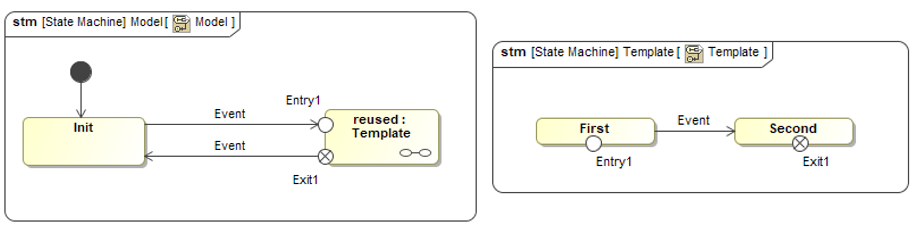
\includegraphics[keepaspectratio, width=150mm]{figures/statechart_elements/SubmachineState.png}
	\caption{Állapottérkép újrafelhasználása Submachine State segítségével}
	\label{fig:SubmachineState}
\end{figure}
\linebreak Logikailag állapotátmenetek is összetartozhatnak, ezért célszerű bizonyos esetekben egyesíteni, vagy szétbontani őket több alternatív átmenetre.
\begin{itemize}
	%-------------
	% Csomópont
	%-------------
	\item \emph{Csomópont (Junction)}: pszeudoállapot, több állapotátmenet összekapcsolása és egyként kezelése, például ha a cél állapotuk ugyan az és logikailag összetartoznak vagy egy beérkező átmenet szétbontása több átmenetre. Ilyenkor lehetőség van őrfeltételt rakni az átmenetekre, ezeknek a kiértékelése viszont még azelőtt történik, hogy bármelyik átmenet végrehajtásra kerülne, ezért egy ilyen ágat szokás \emph{statikus feltételes ág}nak nevezni.
	%------------
	% Elágazás
	%-----------
	\item \emph{Döntés (Choice)}: hasonló mint a csomópont, viszont az őrfeltételek az elágazásba való belépéskor értékelődnek ki \emph{dinamikus}an. Ezt jellemzően alternatív útvonalak megadására használjuk, hasonló mint a programozási nyelvekben \emph{"if than else"} elágazás. Fontos megjegyezni, hogy az elágazás és a csomópont esetében is lehetséges, hogy több átmenet is tüzelhetne, ilyenkor az érvényre jutó átmenet kiválasztása nem determinisztikus módon történik ezért elkerülendő, például \emph{else} őrfeltétel alkalmazásával.
	
	A csomópont szintaxisa egy a kezdő állapotnál kisebb színezett kör, a döntésé pedig egy rombusz. (\ref{fig:choice-junction} ábra).
	
	%-----------------
	 %Ábra

	\begin{figure}[!ht]
		\centering
		\fbox{
\includegraphics[keepaspectratio, width=70mm]{figures/choice.png}}\vspace{1cm}	
		\fbox{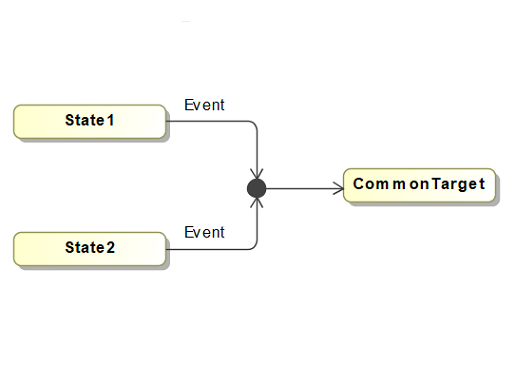
\includegraphics[keepaspectratio, width=70mm]{figures/junction.png}}
		\caption{Döntés és Csomópont szintakitkája}
		\label{fig:choice-junction}
	\end{figure}

	
	
	
\end{itemize}

\section{Eclipse Modelling Framework}
Az Eclipse egy nyílt forráskódú platform független keretrendszer és fejlesztőkörnyezet ami kiterjeszthető, hogy Java mellett más programnyelveket(pl. C, PHP, Ruby, Python, Erlang) is támogasson, de modellező eszközként is használható (pl. Yakindu, Papyrus, Gamma).

Az Eclipse Modelling Framework (EMF) Eclipse plug-inok egy halmaza, amik lehetővé teszik adatmodellek létrehozását és ebből kód generálását. Az EMF kétféle modellt különböztet meg a meta-modellt és példány modellt. A példány modell struktúráját a meta-modell írja le. A modell egy konkrét példánya a meta-modellnek.

Az Eclipse Modelling Framework  működése meglehetősen komplex ezért részletes bemutatása nem célja a dolgozatnak (szakirodalom a keretrendszer kapcsán: \emph{EMF: Eclipse Modelling Framework}\cite{steinberg2008emf}), csak azoknak az alap fogalmakat és működési mechanikáknak az ismertetésre amik szükségesek a dolgozat megértéséhez.

Egy EMF meta-modell \verb+ecore+ és egy \verb+genmodel+ leíró fájlból áll. Előbbi magát a modellt utóbbi pedig a modell generálására vonatkozó információkat tartalmaz. Az \emph{EMF persistence framework} lehetővé teszi modellek perzisztens tárolását XMI és XML alapokon. A fájlrendszerben található modelleket \emph{Resource}-ok reprezentálnak melyeket egy URI séma azonosít. A \emph{Resource}-ok \emph{ResourceSet}-ekbe helyezhetők. A modellek közötti hivatkozások feloldásához a modelleket tartalmazó \emph{Resource}-oknak azonos \emph{ResourceSet}-ekben kell lenniük.

Eclipses környezetekben az EMF-nek nagy jelentősége van. Xtext\footnote{Xtext: https://www.eclipse.org/Xtext/}-el együtt alkalmazva saját szakterület specifikus nyelveket lehet fejleszteni saját nyelvtannal és absztrakt szintaxissal.

\section{MagicDraw}
A MagicDraw a No Magic \cite{NoMag} nevű cég által fejlesztett modellező eszköz, amivel a modellek előállításán kívül lehetőségünk van ezeket szimulálni, validálni, vagy akár kóddá alakítani. Az eszköz első sorban UML modelleket lehet készíteni, de plug-innal lehetőségünk van SysML \cite{SysML} modelleket is létrehozni. Ehhez egy az eszköz fejlett grafikus felhasználói interfészt biztosít (\ref{fig:mdgui}. árba), amivel gyorsan és hatékonyan tudunk modelleket létrehozni. 

A SysML egy általános-célú modellezési nyelv ami az UML egy részének kiragadásával és annak kibővítésével keletkezett. SysMLel struktúrát és viselkedést lehet leírni magas szinten. Alapeleme a Blokk, ami UML-ben a Classnak felel meg. A Blokk egy absztrakt egység ami bárminek megfeleltethető, így a modellezendő rendszer is általában egy Blokként jelenik meg. A Blokkok definícióját és tartalmazási hierarchiáját Block Definition Diagramokkal írhatjuk le. Egy másik megemlítendő diagramfajta az Internal Block Diagram, amivel a Blokkok belső felépítését és komponenseinek kapcsolatait lehet leírni portok segítségével.

Viselkedést Állapottérképekkel és Activity Diagrammokkal szokás leírni SysMLben. Utóbbival munka- és adatfolyamokat, ahol a folyamat lépései \emph{Activity}k és \emph{Action}ök. Állapottérképekkel reaktív rendszereket szokás leírni, a rendszer eseményekre reagál, ezek határozzák meg a viselkedését, szemben az Activity Diagrammokkal, amivel adott bemenetből valamilyen kimenet előállításának folyamatát írjuk le.

\begin{figure}
	\centering
	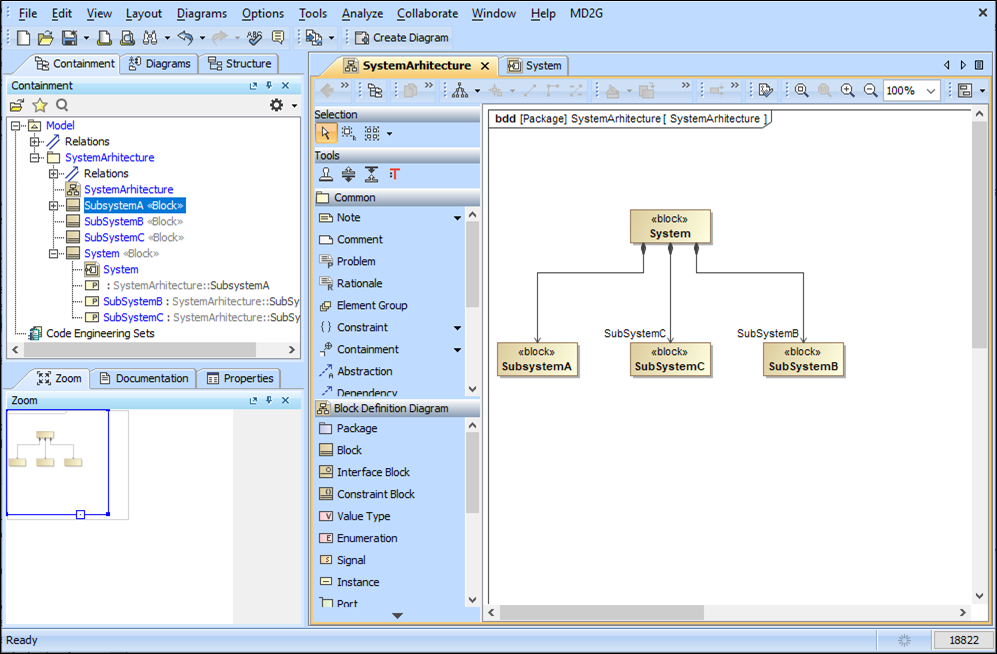
\includegraphics[keepaspectratio, width=150mm]{figures/magicdrawgui.png}
	\caption{MagicDraw felhasználói felülete}
	\label{fig:mdgui}
\end{figure}

\subsection{Állapottérképek SysMLben}
Az állapottérképeket SysML modellek részeiként, más modell elemekhez vannak viselkedésként hozzárendelve, a triggereket aktiváló események a modell strukturális leírásában vannak definiálva, az elvégezhető akciók pedig más modell elemek által leírt viselkedések. Mivel a dolgozat kizárólag állapottérképekkel foglalkozik ezért implicit feltételezzük, hogy az állapottérképen használt szignálok definiálva vannak és ezeket az állapotgép fogadni tudja, azaz rendelkezik a megfelelő portokkal és interfészekkel amelyek ezt lehetővé teszik.

\subsection{Plug-in fejlesztése MagicDrawhoz}
A MagicDraw lehetővé teszi, hogy harmadik fél plusz funkciókat adhasson az eszközhöz plug-inok formájában. A MagicDraw Java nyelven íródott, plug-int is ezen a nyelven van lehetőség fejleszteni, ehhez egy Api-t kapunk amit Open Api-nak \cite{OpenApi} hívnak, ez teszi lehetővé, a modell elemek kóddal történő manipulációját, és a grafikus interfész kiegészítését, saját funkcionalitással.

A MagicDraw indulásakor bejárja a plug-in könyvtárat plug-in leíró fájlokat tartalmazó könyvtárak után. Ezek írják le melyik Java osztály reprezentálja a plug-int, ennek le kell öröklődnie a \emph{com.nomagic.magicdraw.plugins.Plugin} osztályból. A MagicDraw plug-ins managere meghívja ennek az osztálynak az init metódusát, amiben GUI elemeket tudunk regisztrálni, vagy egyéb funkcionalitást hozzáadni az eszközhöz.

\lstset{style=javacode}
\begin{lstlisting}
public class MyPlugin extends com.nomagic.magicdraw.plugins.Plugin {

	public void init(){
		//plugin belépési pontja
	}
	
	public boolean close(){
		//plugin leáll
	}
	
	public boolean isSupported(){
		//feltételek teljesülése a plug-in betöltéséhez
		return true;
	}
	
}
\end{lstlisting}

A SysML elemei sztereotipizált UML elemek, a SysML plug-in SysML szintaktikát használ, de a létrehozott elemek a MagicDraw UML meta-modellje szerint lesznek példányosítva megfelelően sztereotipizálva, ezért kód szinten is eszerint érhetőek el.

A modell elemek ugyan saját MagicDraws implementációval rendelkeznek, de EMF \footnote{Eclipse Modelling Framework https://www.eclipse.org/modeling/emf/}-es interfaceket is realizálnak ezért lehetőségünk van EMF Apijának használatára a plugin fejlesztése során.

\section{Viatra}

Az Eclipse Viatra Framework\footnote{Viatra: https://projects.eclipse.org/projects/modeling.viatra} egy Eclipse alapú keretrendszer ami lehetővé teszi modellek hatékony eseményvezérelt transzformációját és lekérdezését. A modell lekérdezésekhez egy külön nyelvet Viatra Query Language(VQL)-t használ. VQL lekérdezésekből Java osztályok generálódnak: ezek a lekérdezek java kódbeli reprezentációi, melyek felhasználása lehetővé teszi modell transzformációk hatékony implementációját és a lekérdezésekre illeszkedő elemek lekérdezését a modellből.

Viatra használatában MagicDraw plugin fejlesztése során is van lehetőség. A Viatra for MagicDraw (V4MD) egy plug-in ami lehetővé teszi a Viatra Api használatát más plug-inokban. A V4MD projekt megnyitásakor létrehozza azokat a VIATRA specifikus objektumokat amelyeken keresztül lekérdezéseinkkel hozzá férhetünk a MagicDraw projekt modelljeihez.

\section{Formális verifikáció}
\label{sec:formal-verif}
A modell alapú fejlesztés egyik nagy előnye, hogy már tervezési fázisban tudjuk vizsgálni rendszerünk egyes aspektusait. A rendszer helyes működésének ellenőrzését verifikációnak hívják. Ez történhet tesztekkel, szimulációval, vagy formális módszerekkel.

A formális módszerek előnye, hogy a rendszer helyességéről matematikailag precíz bizonyítást adnak, nem szükséges az elvárt kimenetek meghatározása, csak megkötések megfogalmazása. Továbbá teljesek ezért nem kell lefedettséggel foglalkozni mint tesztelésnél. Megkötés sérülésekor, vissza lehet követni, azt végrehajtási útvonalat(\emph{execusion trace}) ami a megszorítás megsértéséhez vezetett. Hátrányuk, hogy nehezen skálázható, erőforrás igényes és egy összetett rendszert formális módszerekre való visszavezetése gyakran nehézkes.

Állapottérképek formális verifikációjára már léteznek megoldások. A Gamma keretrendszer például képes állapottérképek verifikációjának elvégzésére. Ehhez az Uppaal \cite{bengtsson1995uppaal, bengtsson1998new} nevű eszközt használja fel.

\section{Gamma Framework}
\label{sec:gamma-framework}
A Gamma Statechart Composition Framework komponens alapú reaktív rendszerek tervezésére, validálására, verifikálására és kód generálásra lett létrehozva. Az eszköz alap komponensei az állapottérlépek amiknek a leírásához egy saját nyelvet Gamma Statechart Languaget (\ref{fig:gamma-syntax}. ábra) definiál, ami lehetővé teszi külső modellező eszközök integrálását is. Az első integrált eszköz a Yakindu Statechart Tools \cite{toolsyakindu}, aminek a modelljeit Gamma képes a saját maga által definiált modellekké (\ref{fig:gamma_statechart_model}. ábra) transzformálni és feldolgozni.

Az eszköz egy másik komponensei az ún. Kompozit komponensek, amiket Gamma Composition Languagel lehet definiálni. Ezek írják le a rendszer felépítését komponensekre bontva, illetve az ezek portjai és interfészei között definiált kapcsolatokat.

A keretrendszer még két saját nyelvet definiál. Az egyik a Gamma Constraint Language amivel megszorításokat lehet definiálni, ami egy általános megoldása típus definíciók, változók, függvények deklarálásához és kifejezések specifikálásának.

A másik nyelv pedig Gamma Interface Language, ami interfészek definiálását teszi lehetővé, amik a kapcsolódó komponensek egymás felé nyújtanak. Az interfész határozza meg, hogy milyen események fogadhatóak, vagy küldhetőek. Ezek az interfészekben deklarálandók és irányuk lehet, \emph{IN, OUT, INOUT}.

Munkámban a egy MagicDraw plug-int hozok létre ami a formális verifikáció végrehajtásához a Gamma keretrendszert használja azáltal, hogy \emph{VIATRA} segítségével áttranszformálja a MagicDraw modelljeit Gamma modellekké.

\begin{figure}[!ht]
\begin{lstlisting}
package Exapmle

statechart MonitorStatechart [] {

transition from Red to Blue
transition from Entry0 to Red

	region main_region {
		initial Entry0
		state Red
		state Blue
	}
}
\end{lstlisting}
\caption{Gamma Statechart konkrét szöveges szintaxisa}
\label{fig:gamma-syntax}
\end{figure}


\begin{figure}[!ht]
	\centering
	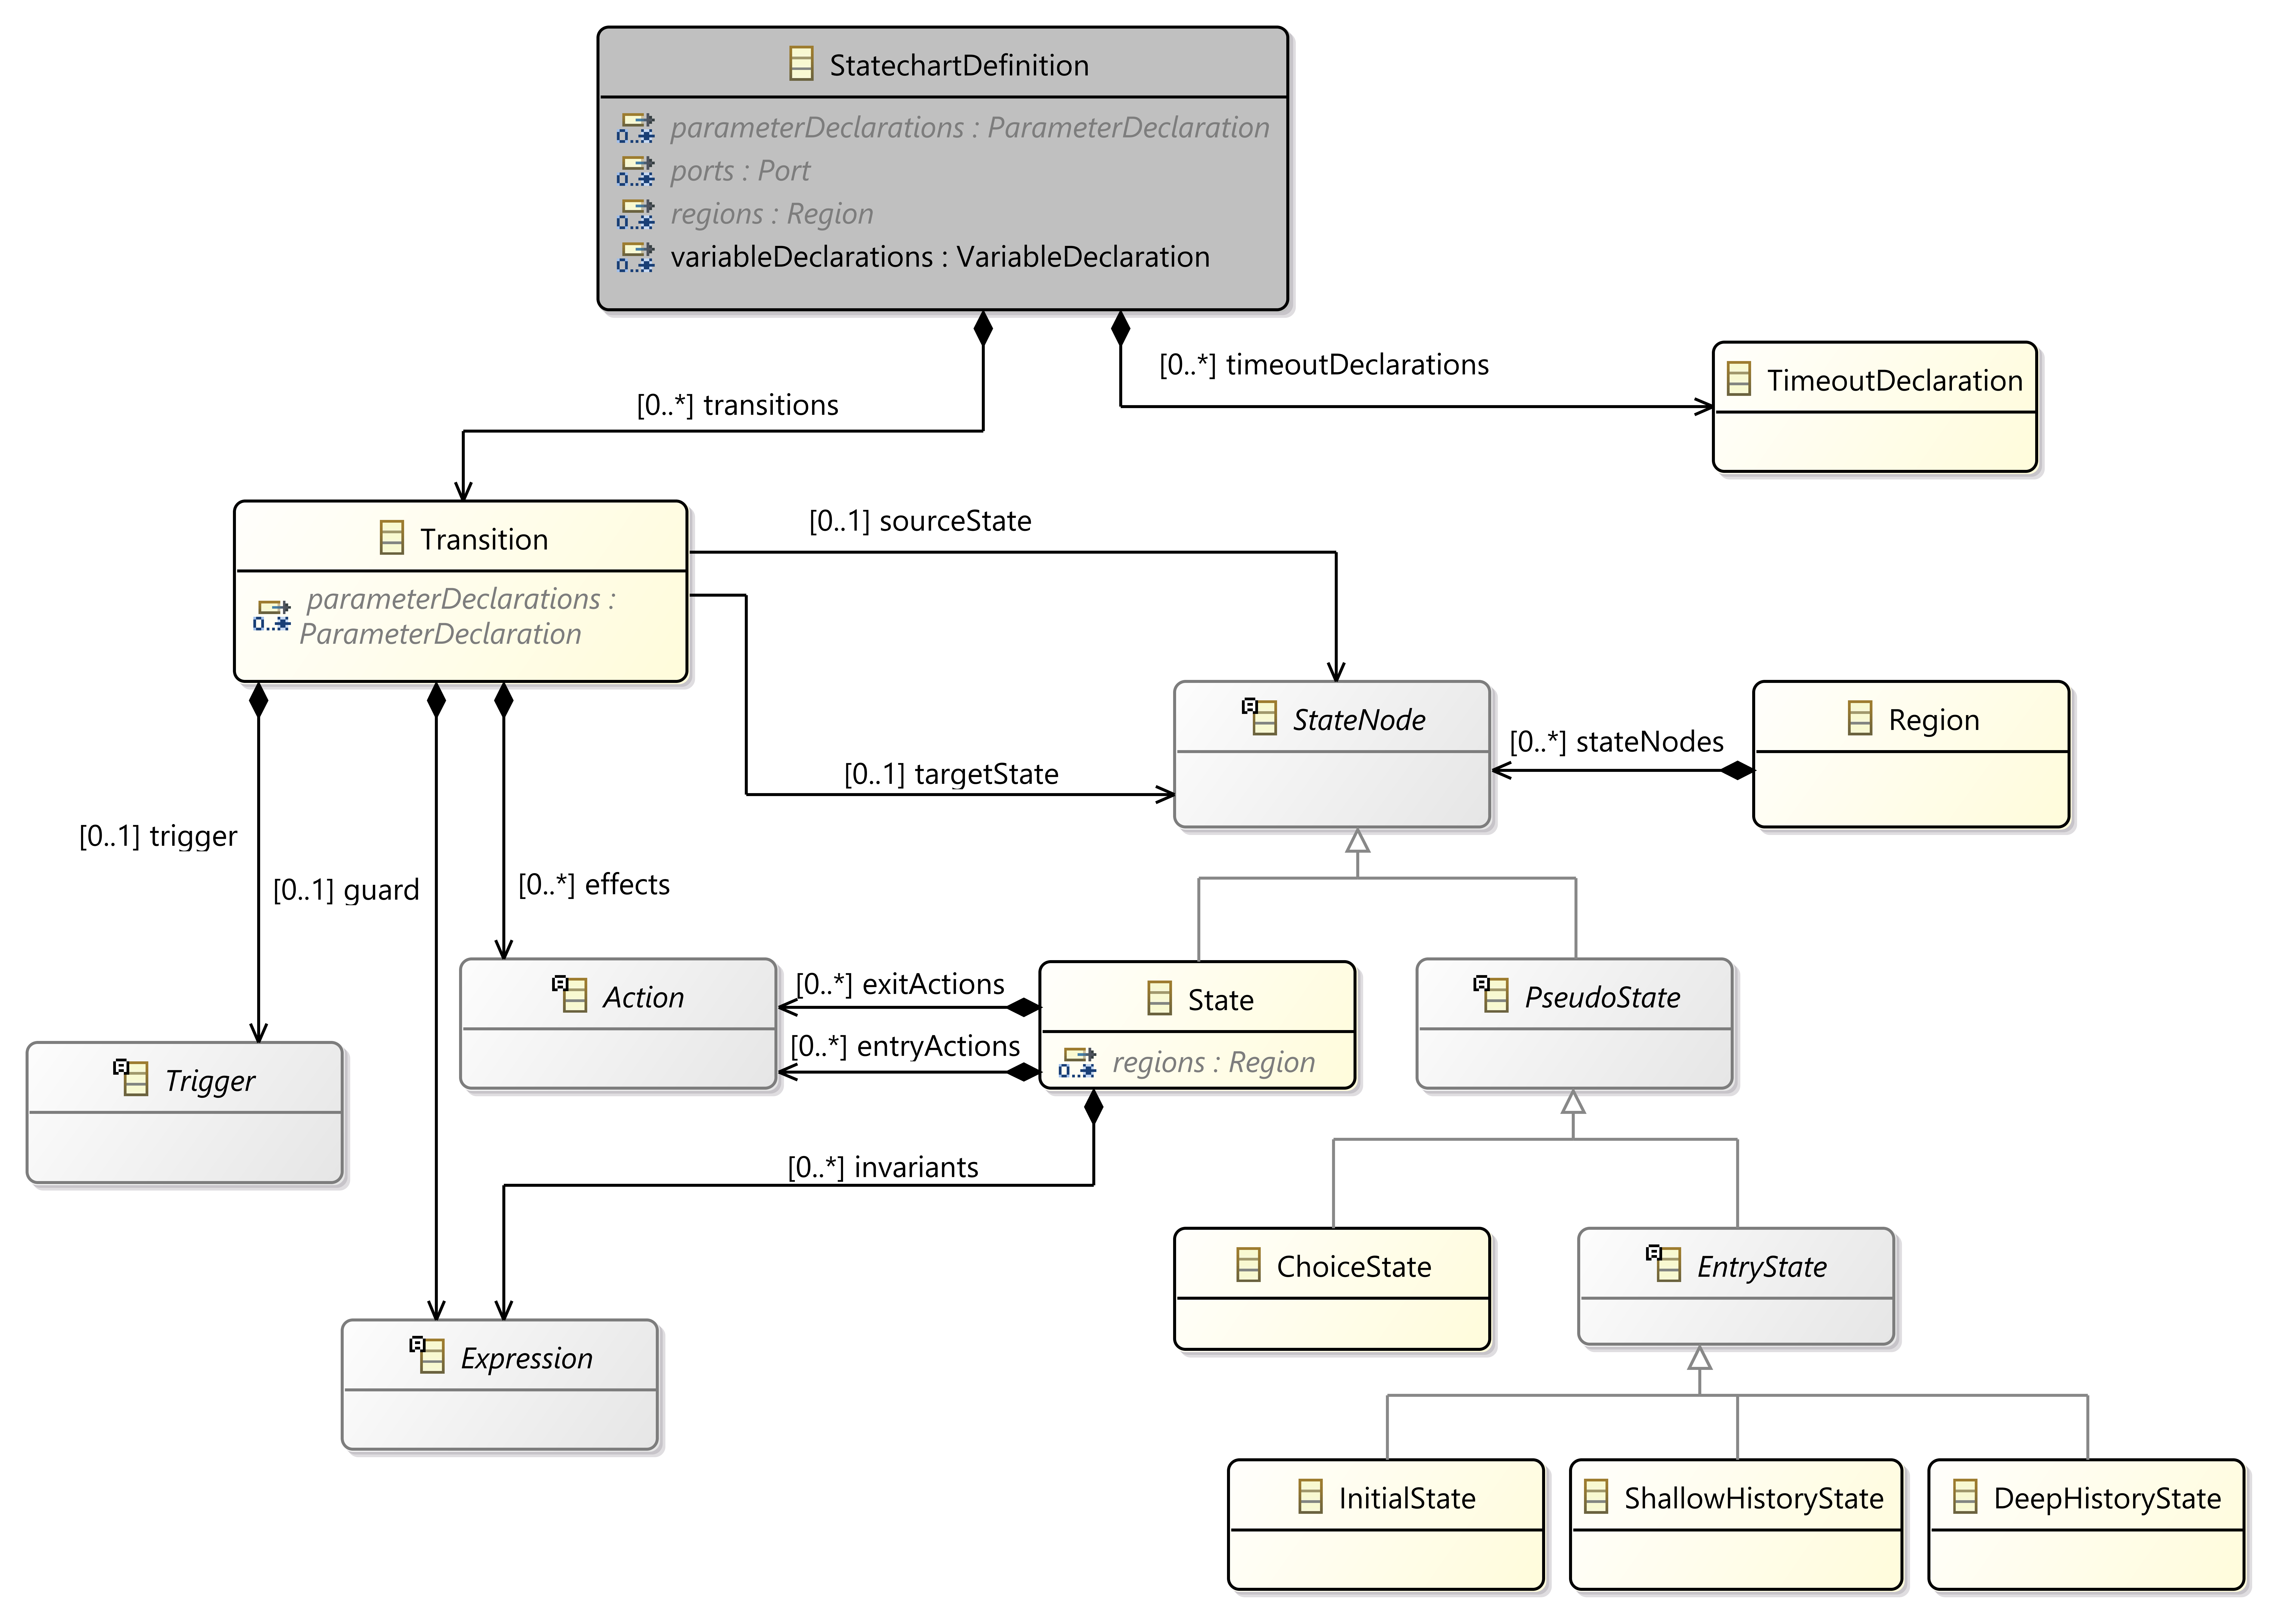
\includegraphics[keepaspectratio, width=150mm]{figures/statechart_class_diagram.png}
	\caption{Gamma állapottérkép absztrakt szintaxisa}
	\label{fig:gamma_statechart_model}
\end{figure}



